\chapter{System Design}
This chapter will provide a detailed description of the system’s overall design. It will begin by providing an overview of the system’s architecture before providing a detailed discussion of the main constituent parts that make up the system. 

\section{System Architecture} 
An iPhone and Android-compatible cross-platform mobile application is included in the system architecture's design. A Node.js server is added to the MySQL database that serves as the system's foundation. Additionally, a cross-platform mobile framework was used to construct the frontend components. Internet connectivity enables communication between the various components, enabling users to access and interact with the programme without any difficulty. The architecture illustration can be seen in Figure \ref{image:architecture}.
\begin{figure}[h!]
    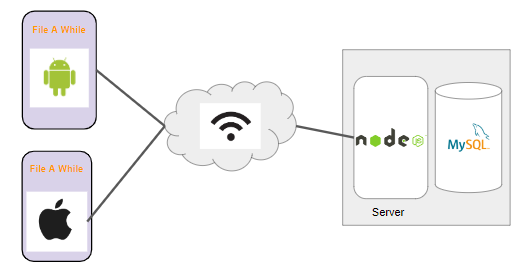
\includegraphics[width=0.7\textwidth]
    {images/Architecture.png}
    \centering
    \label{image:architecture}
    \caption{Architecture}
\end{figure}

\section{Application Design}
The login screens and navigation system screens are two essential parts of the application design. The developer created a set of wireframes to mockup the set of required screens before starting the app development process which enabled careful planning of the system design, which is visually represented in Figure \ref{image:wireframe}. The use of wireframes allows quick development since it makes it easier to comprehend the frontend components that are needed and where they should be placed and how the user navigates between them.
\begin{figure}[h!]
    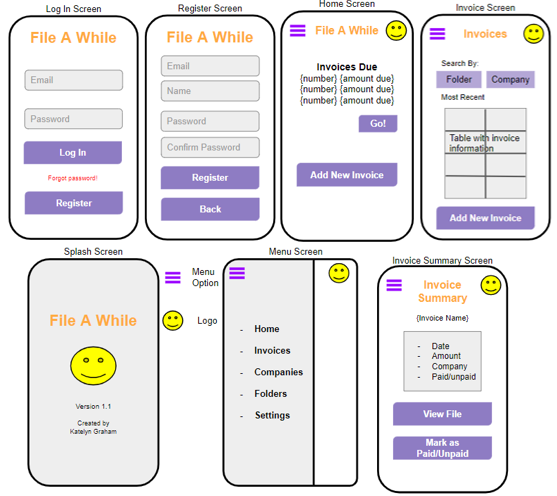
\includegraphics[width=1.0\textwidth]
    {images/AllWireframes.png}
    \centering
    \label{image:wireframe}
    \caption{Wireframes}
\end{figure}

\subsection{Authentication}
The Registration Screen and the Login Screen are two separate screens that make up the authentication screens. The application also includes a splash screen, which is prominently displayed when it is first launched, as seen in Figure \ref{image:splash}. The Splash screen includes a brief display of the application name, creator, and version number along with an image of the app logo, Figure \ref{image:logo}. In order to achieve a smooth transition to the succeeding panels, a standard loader display is used for the entirety of the splash screen.
\begin{figure}[h!]
    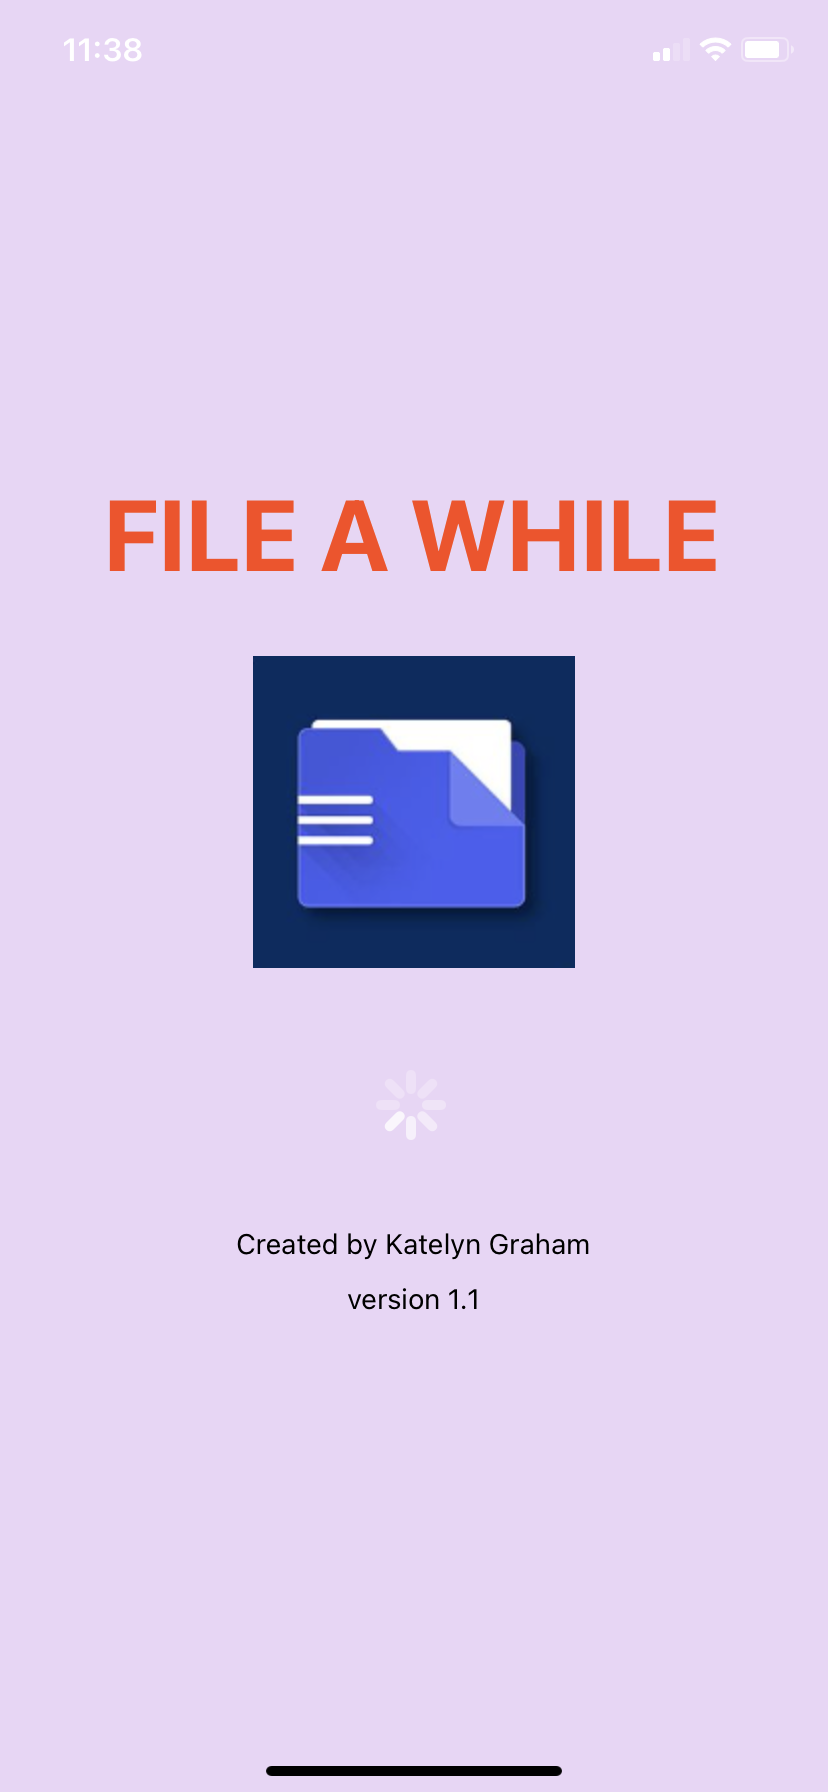
\includegraphics[width=0.3\textwidth]
    {images/SplashScreen.png}
    \centering
    \label{image:splash}
    \caption{Splash Screen}
\end{figure}

\begin{figure}[h!]
    
\includegraphics[width=0.2\textwidth]
    {images/FileLogo.png}
    \centering
    \label{image:logo}
    \caption{App Logo}
\end{figure}

\subsection{Login Screen}
The log-in interface, Figure \ref{image:login}, is straightforward to avoid confusing the user. To access their account, the user only needs to provide their email address and password. If the user does not currently have an account, they can create one by clicking the Register link that appears beneath the login button, which will direct them to the registration page. 
\begin{figure}[h!]
    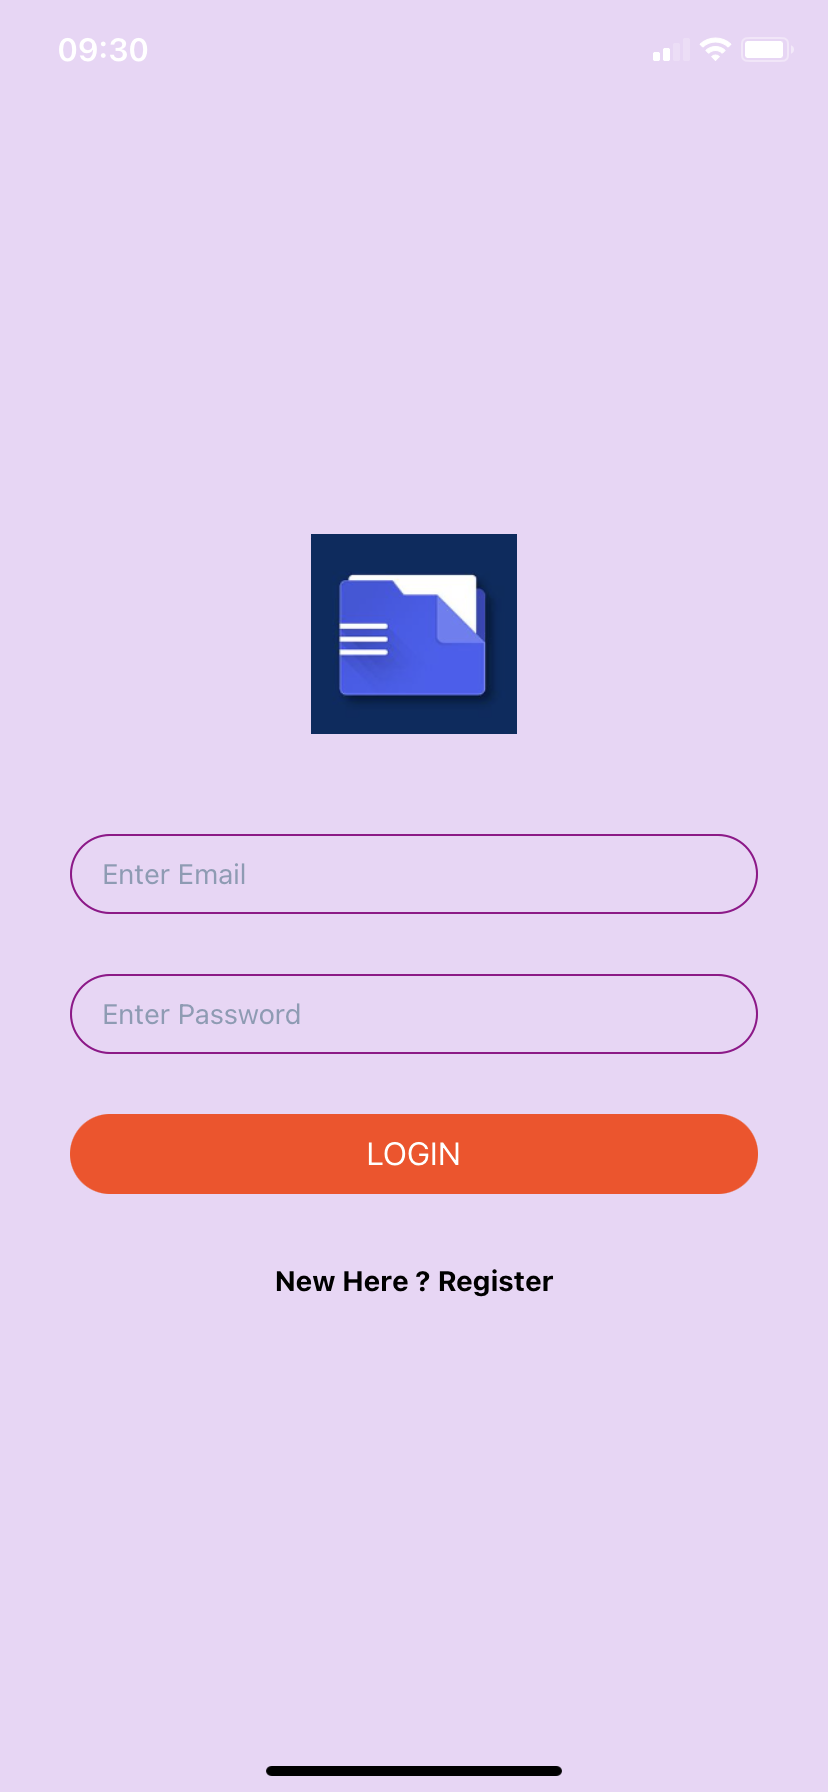
\includegraphics[width=0.3\textwidth]
    {images/Login.png}
    \centering
    \label{image:login}
    \caption{Login Screen}
\end{figure}

\subsection{Registration Screen} 
Figure \ref{image:registeration} shows the Registration Screen, which resembles the Login Screen but also includes a name entry box in addition to the email and password input fields. Users will be taken to the Registration Successful Screen, seen in Figure , after clicking the register button and assuming all required fields have been filled out correctly. They can select a button to enter the Login Screen from this location. An alert box will show if a user fails to complete any of the required registration fields, directing them to take the appropriate corrective action.
\newline \newline
A user will be asked to save their password to their Keychain when signing up for an iPhone. By providing face ID for quick and smooth login authentication, this functionality streamlines and accelerates the login process.
\begin{figure}[h!]
    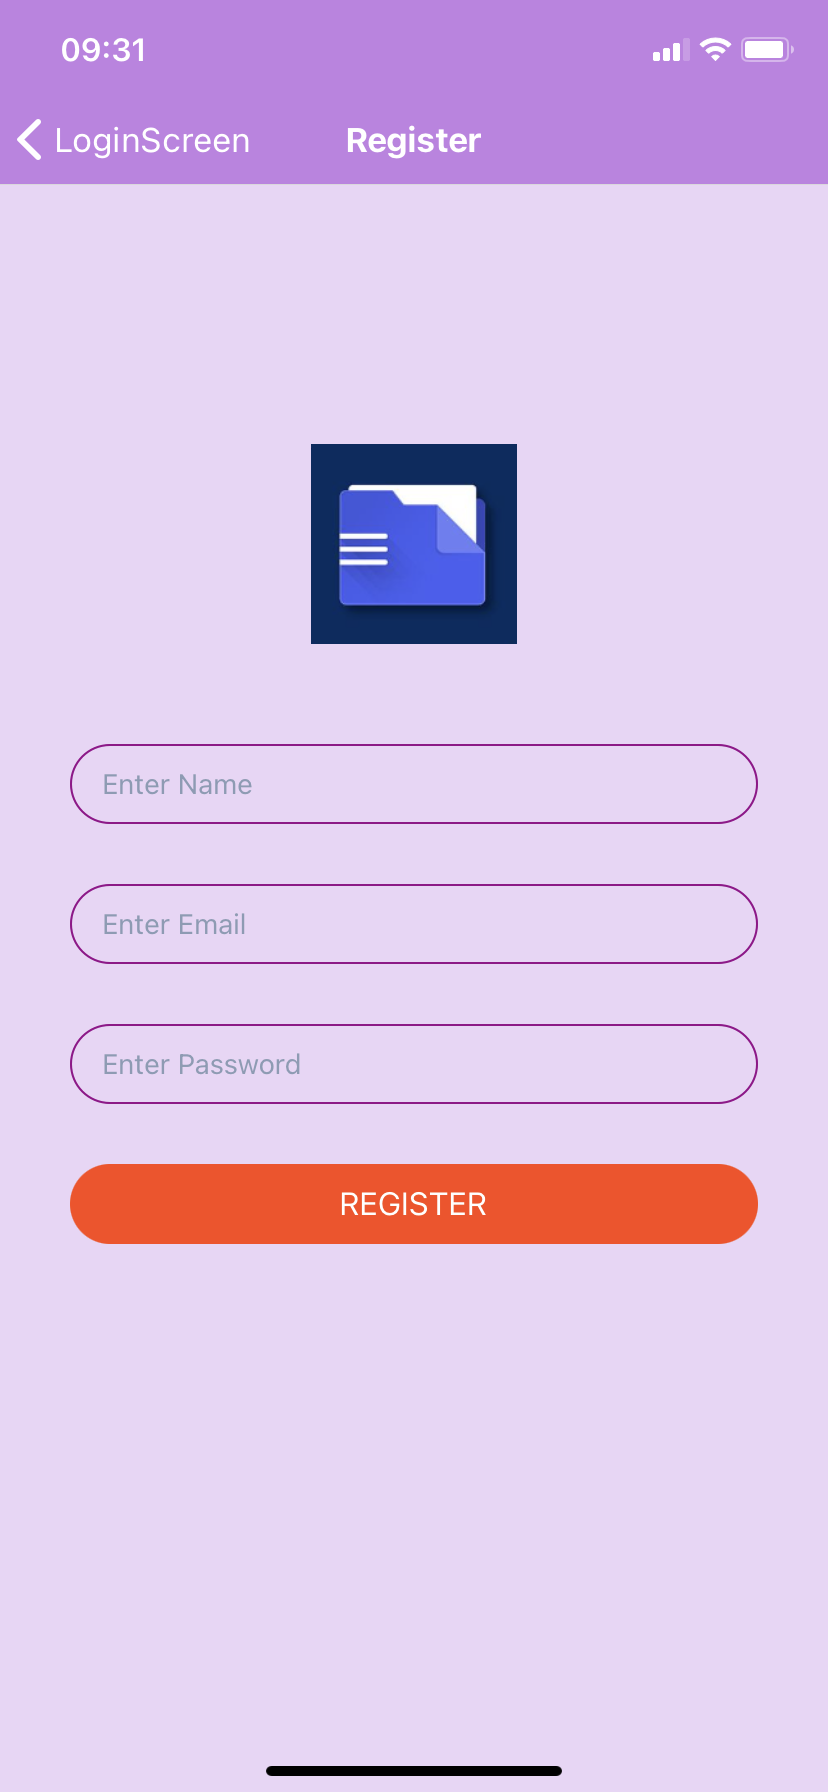
\includegraphics[width=0.3\textwidth]
    {images/Registration.png}
    \centering
    \label{image:registeration}
    \caption{Registration Screen}
\end{figure}
\begin{figure}[h!]
    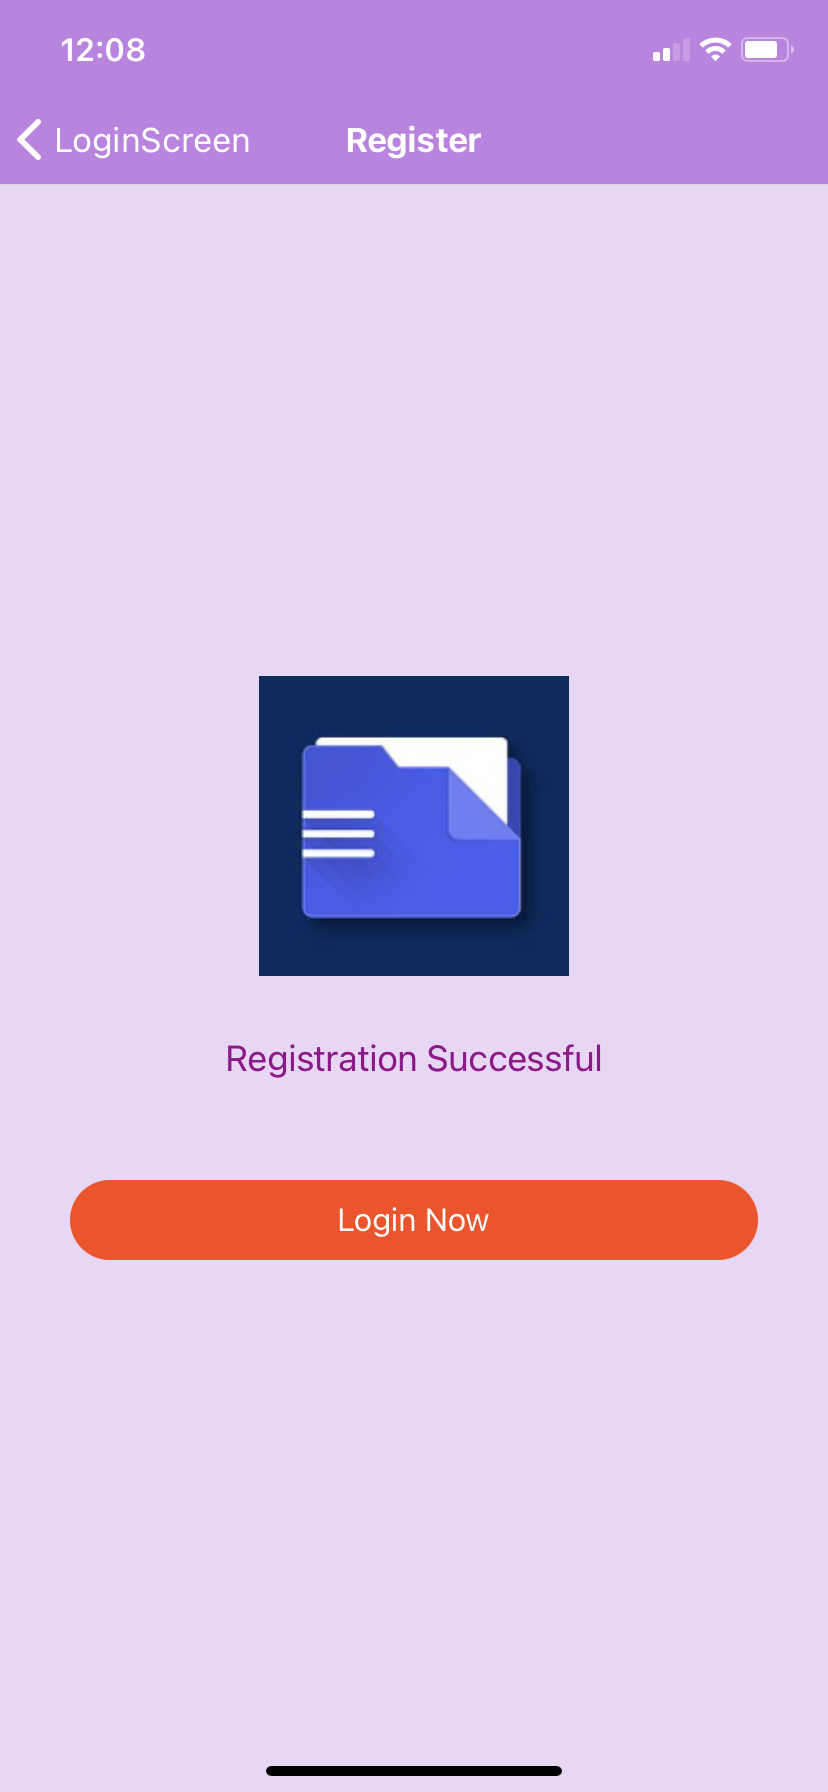
\includegraphics[width=0.2\textwidth]
    {images/RegSuccess.png}
    \centering
    \label{image:regsuccess}
    \caption{Successful Registeration Screen}
\end{figure}

\subsection{Navigation}
The carefully thought-out Drawer Navigation System, shown in Figure \ref{image:nav}, has been created to offer users a handy side menu that can be quickly accessed by swiping from the left edge of the screen or by clicking on the menu symbol located in the upper left corner. The side menu includes a set of options allowing the user to navigate to specific sections of the Application. Users enjoy a simple and efficient navigation process due to the fast presentation of the appropriate screen after selecting a particular item in the menu.
\begin{figure}[h!]
    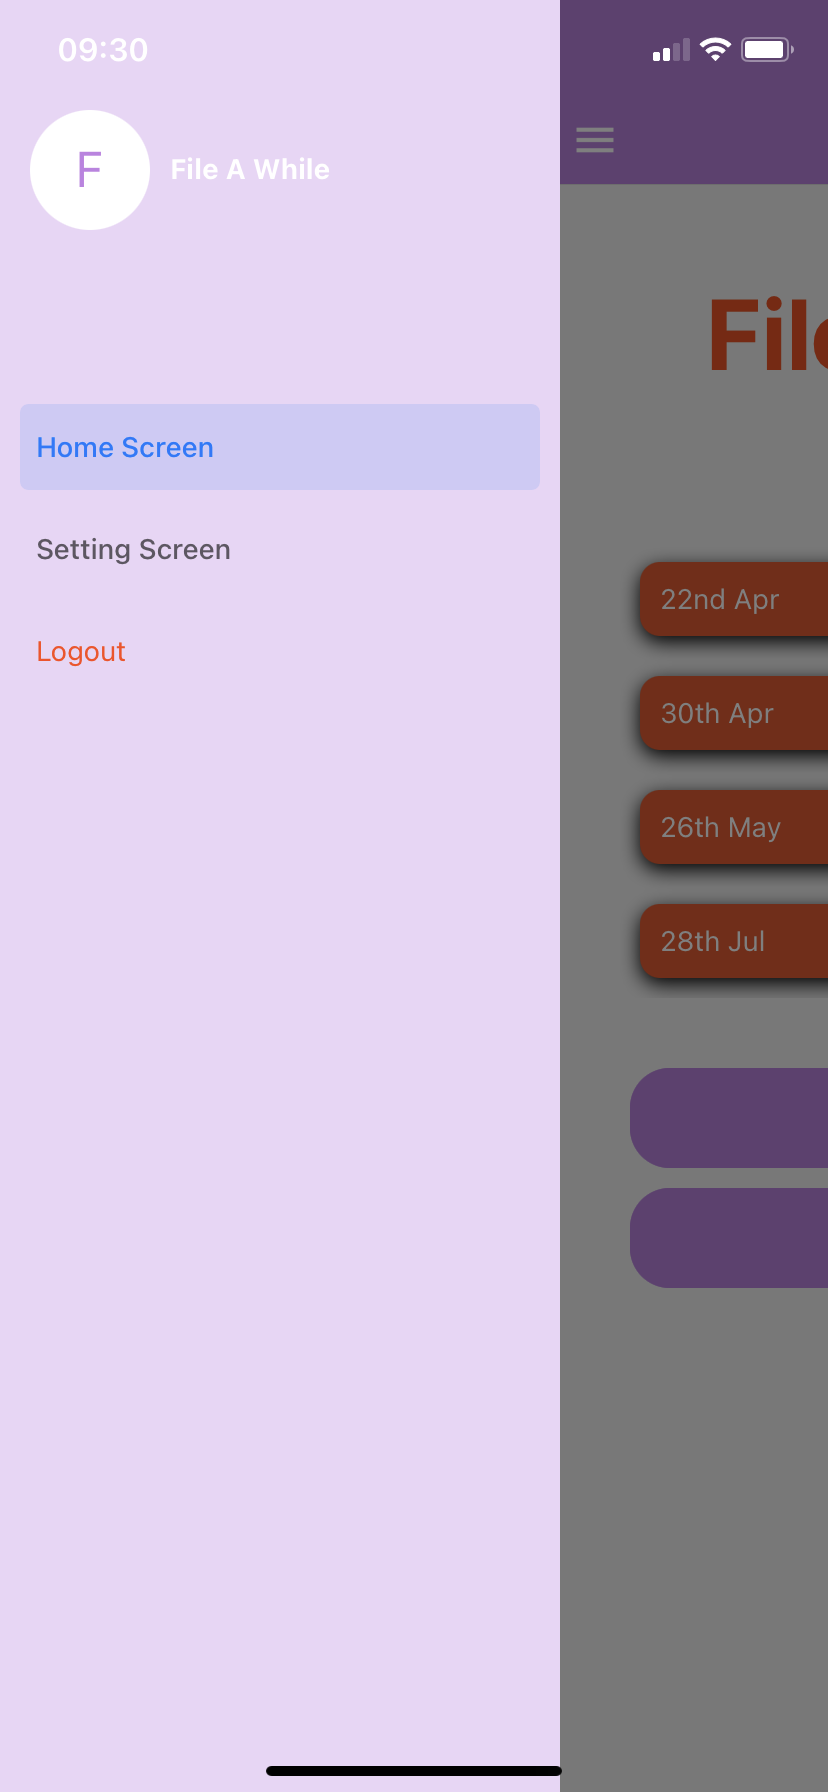
\includegraphics[width=0.3\textwidth]
    {images/Nav.png}
    \centering
    \label{image:nav}
    \caption{Drawer Navigation}
\end{figure}

\subsection{Home Screen}
The Home Screen, \ref{home} which is the user's first screen after logging in, serves as the application's main area. It includes a scrollable list of unpaid invoices, each of which is touchable and, upon selection, takes users to an informative Invoice Summary Page. This page gives a summary of the invoice, including its name, amount, and other important details. Invoices can be marked as paid or completely deleted by users, allowing for effective invoice administration. A back button in the page's upper left corner makes it simple to return to the Home Screen.
\newline \newline
There are two different buttons, each with a different function, underneath the scrollable list. Users who click the first button “Add New Invoice” are taken to a page \ref{allinvoice} that resembles the Home Screen but features a scrollable list that shows every invoice, paid and unpaid. Users can create new invoices on that page by clicking the “Add New Invoice” button. On the Create Invoice screen \ref{create}, the amount and company name of the invoice must be entered, and users can choose a date in the date picker to enter the due date for when the invoice is supposed to be paid. The system will automatically set the due date to the current date if the user forgets to choose one. Additionally, users can change the new invoice's status from unpaid to paid by using the dedicated paid toggle.
\begin{figure}[h!]
    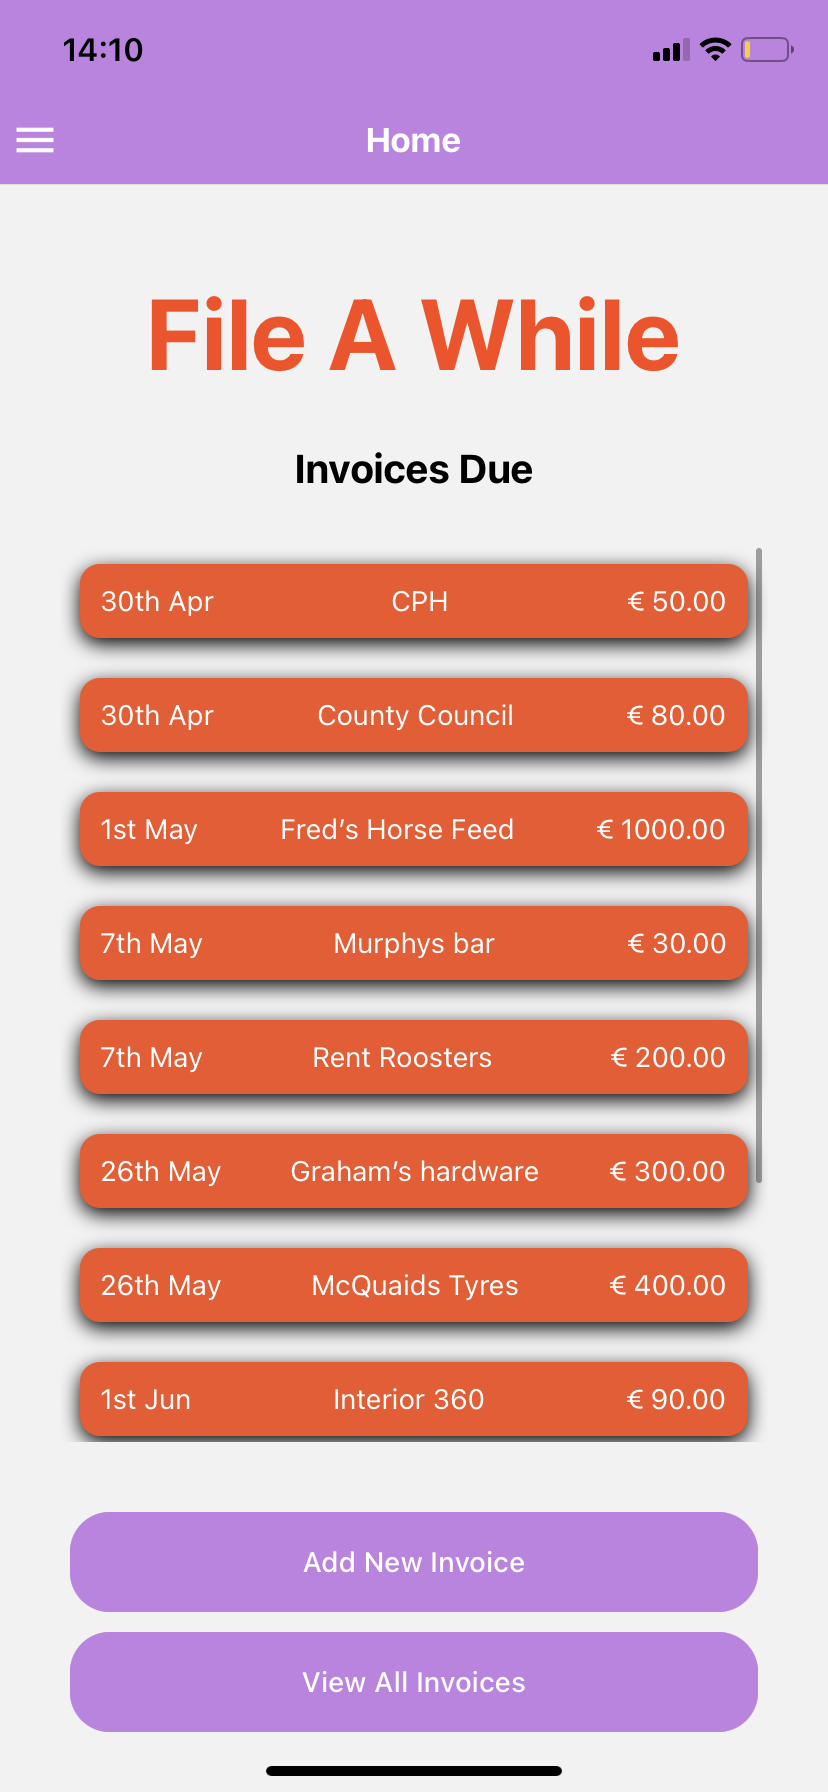
\includegraphics[width=0.3\textwidth]
    {images/Home.png}
    \centering
    \label{image:home}
    \caption{Home Screen}
\end{figure}
\begin{figure}[h!]
    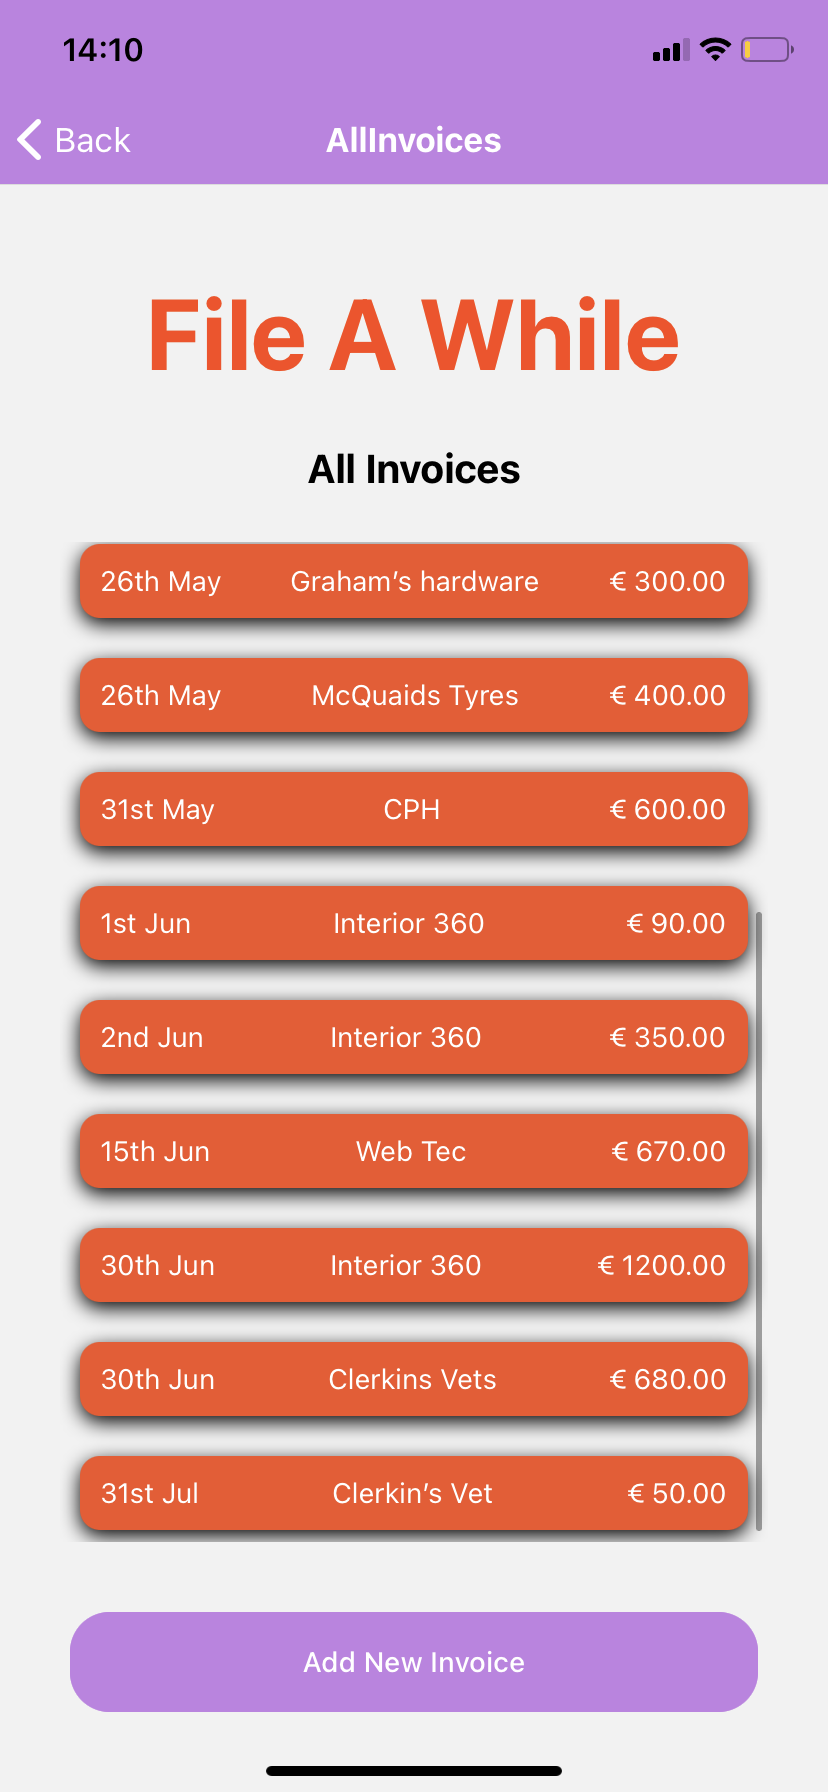
\includegraphics[width=0.25\textwidth]
    {images/AllInvoice.png}
    \centering
    \label{image:allinvoice}
    \caption{All Invoices Screen}
\end{figure}
\begin{figure}[h!]
    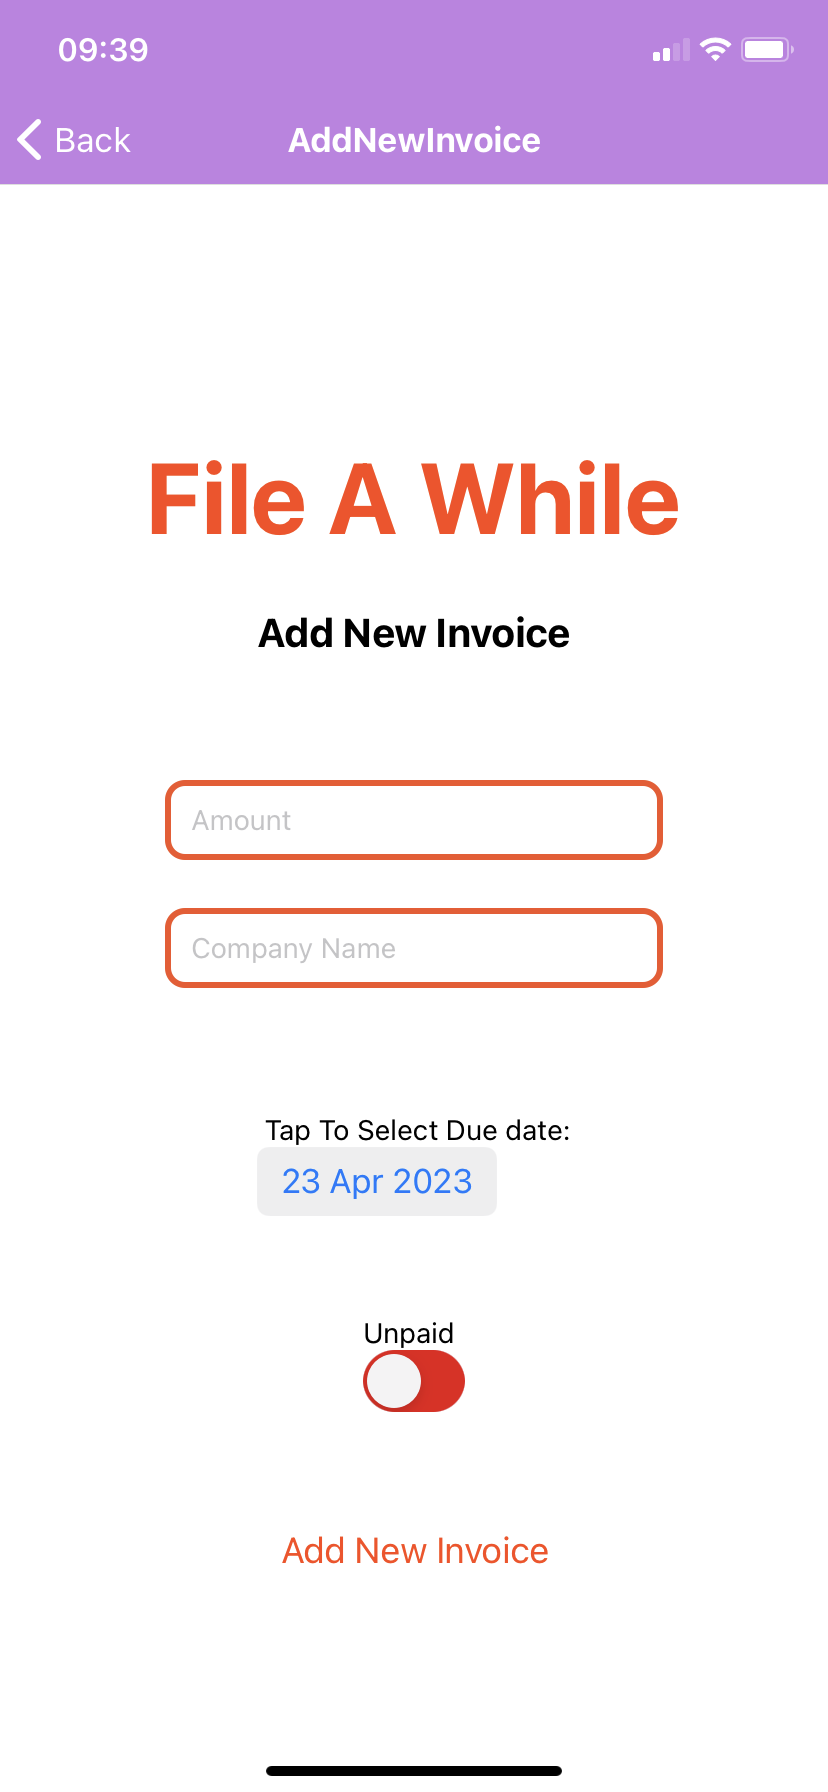
\includegraphics[width=0.25\textwidth]
    {images/Adding.png}
    \centering
    \label{image:create}
    \caption{Add New Invoice Screen}
\end{figure}

\subsection{Settings Screen}
The Settings Screen \ref{setting}, which can be accessed through the Drawer Navigation, gives users the ability to change their account password. Users must be aware of their current password in order to make this change, and they must type in the new password twice while making sure it matches the confirmed password input area. An error message is prominently shown on the screen if users forget their password or enter it incorrectly. It's important to remember that passwords must include a minimum of six characters.
\begin{figure}[h!]
    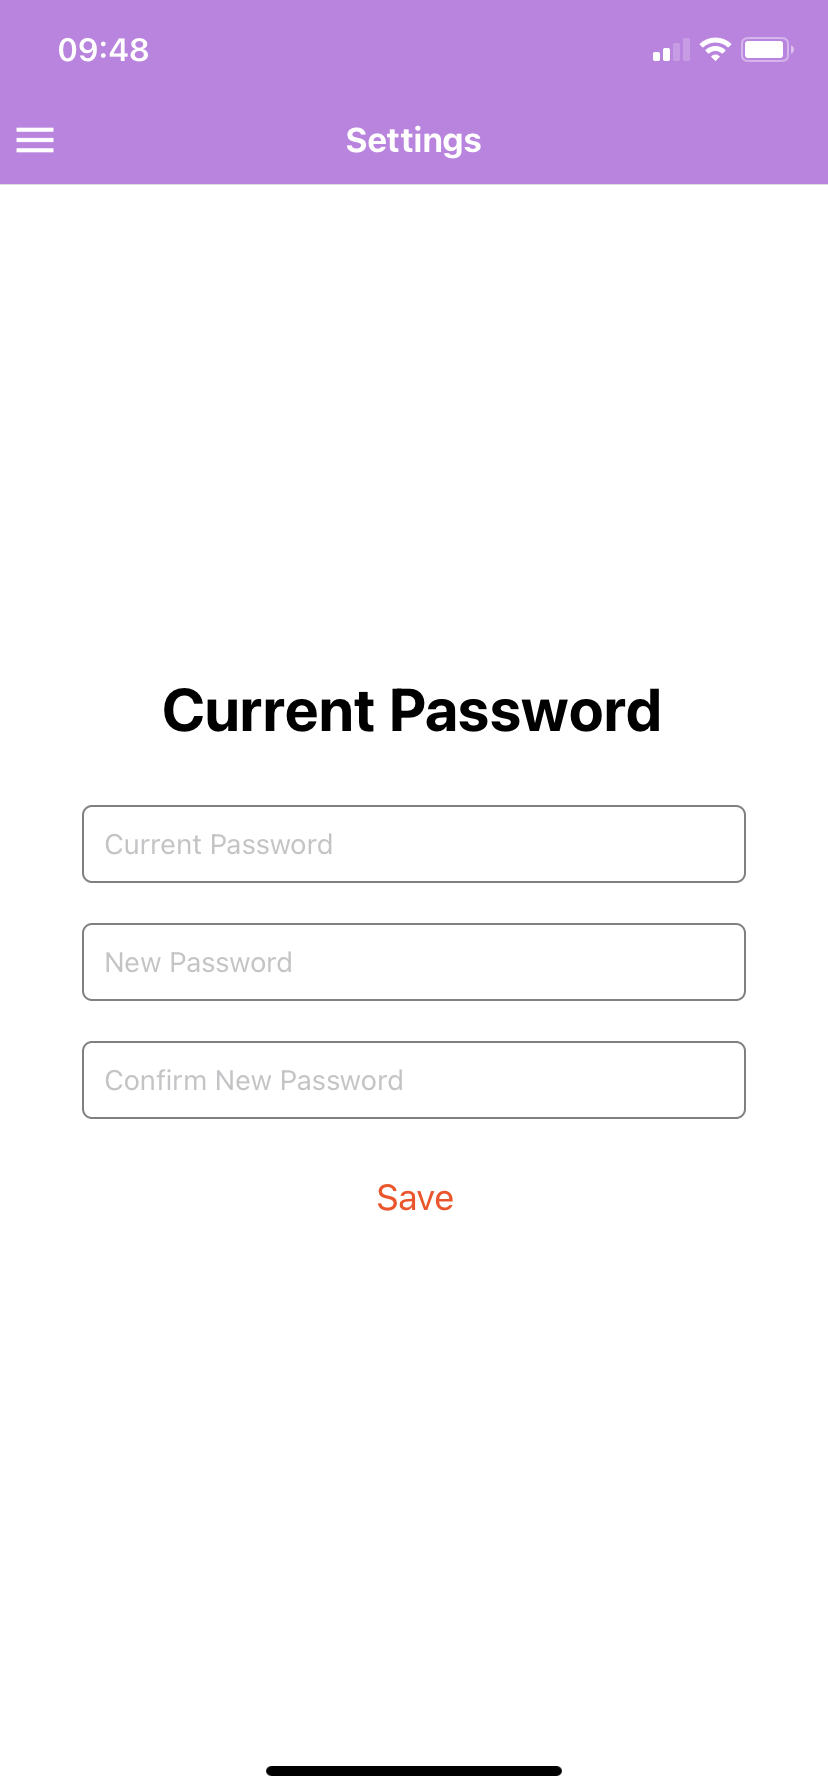
\includegraphics[width=0.3\textwidth]
    {images/Setting.png}
    \centering
    \label{image:setting}
    \caption{Settings Screen}
\end{figure}

